\chapter{Рассчет плана работы на такт.}

\section{Балансировка сборочной линии}

Производственная сборочная линия была впервые представлена
Генри Форд в начале 1900-х годов. Она была разработана, чтобы быть эффективным,
высокопроизводительным способом изготовления конкретного продукта. Базовая сборочная
линия состоит из набора рабочих станций, расположенных линейно, где каждая станция соединена погрузочно-разгрузочным устройством.
Основное движение материала по сборочной линии начинается с того, что деталь подается на первую станцию с
заданной скоростью подачи. Станция считается любой точкой на конвейере, в которой 
выполняется задание с заготовкой. Эти задачи могут выполняться машинами, роботами и
или людьми. Как только деталь поступает на станцию, то для нее выполняется задание, 
и деталь подается на следующую операцию. Время, необходимое для выполнения задачи
в каждой операции, называется временем процесса (Sury, 1971). Время цикла сборочной 
линии определяется желаемой производительностью. Этот уровень производства 
устанавливается таким образом, чтобы желаемое количество конечного продукта 
производилось в течение определенного периода времени (Baybars, 1986). Для того чтобы 
сборочная линия поддерживала определенную производительность, сумма времени обработки
на каждой станции не должна превышать время цикла на станциях (Fonseca et al, 2005). 
Если сумма времен обработки внутри станции меньше времени цикла, говорят, что на этой
станции присутствует время простоя (Erel et al, 1998). Одним из основных вопросов,
касающихся разработки сборочной линии, является порядок организации задач, которые 
необходимо выполнить. Для изготовления любого предмета есть несколько 
последовательностей задач, которые необходимо выполнить. Проблема балансировки 
сборочной линии (ALBP) возникла с изобретением сборочной линии. Хельгесон и др. 
(Helgeson и др., 1961) были первыми, кто предложил ALBP, а Сальвесон (Salveson, 1955)
был первым, кто опубликовал проблему в ее математической форме. 
Однако в течение первых сорока лет существования сборочной линии для балансировки
линий использовались только методы проб и ошибок (Erel et al., 1998). С тех пор 
было разработано множество методов для решения различных форм ALBP. 
Сальвесон (Salveson, 1955) сделал первую математическую попытку, решив задачу в
виде линейной программы. Гутьяр и Немхаузер (Gutjahr и Nemhauser, 1964) показали,
что проблема ALBP относится к классу NP-сложных задач комбинаторной оптимизации.
Это означает, что оптимальное решение не гарантируется для задач значительных размеров. 
Поэтому эвристические методы стали наиболее популярными методами решения проблемы.


Преимущества балансировки линии:

\begin{itemize}
    \item Минимизация количества рабочих станций при заданном цикле
    \item Минимизация цикла при заданном количестве рабочих станций
    \item Минимизация общего времени простоя
    \item Минимизация общего объекта или длины линии
\end{itemize}

Классификация проблемы ALB основана главным образом на целевых функциях и структуре проблемы. Различные версии проблем ALB представлены на рисунке (\ref{ris:image1}).

\begin{figure}[H]
    \center{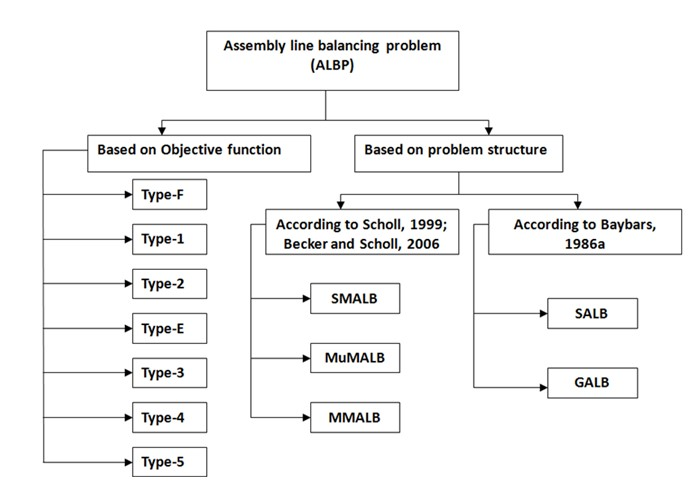
\includegraphics[width=1\linewidth]{fig/Screenshot_1.jpg}}
    \caption{Классификация ALBP}
    \label{ris:image1}
\end{figure}

\subsection{Проблемы базирующиеся на целевых функциях}
В данном подразделе рассматриваются целевые задачи балансировки линии. Далее перечисленные все обозримые проблемы приведенные на классификации \ref{ris:image1} и представленно их краткое описание.
\begin{itemize}
    \item Type F: Рассматривает возможность создание линии при заданном колличестве рабочих станций и цикле.
    \item Type 1: Рассматривает задачу минимизации количества рабочих станций, при фиксированном времени цикла.
    \item Type 2: Рассматривает задачу минимизации времени цикла, при фиксированном количестве рабочих станций.
    \item Type E: Данный тип является самой общей версией ПРТ и рассматривает получение максимальной эффективности линии при минимальном цикле и количестве станций.
    \item Type 3: Рассматривает задачу максимизации плавности рабочей нагрузки.
    \item Type 4: Рассматривают максимизацию рабочей связанности, используется для быстрого производства однотипного продукта.
    \item Type 5: Рассматривает типы 3 и 4 для нескольких продуктов
\end{itemize}

В рамках данной работы рассматривается функция повышения эффективности загрузки. Эффективность сборочной линии подразумевает равную загрузку всех рабочих станций на сборочной линии. 

\subsection{Проблемы основывающиеся на структуре линии}
В данном разделе рассматриваются структурные задачи балансировки линии. Далее перечислены структурные проблемы приведенные на рисунке (\ref{ris:image1}) и их описание.

\begin{itemize}
    \item SMALB: Данная проблема затрагивает структуру, когда на линии производится один тип продукта
    \item MuMALBP: Затрагивает проблемы производства более одного типа продукта партиями на одной линии
    \item MMALBP: Затрагивает производство разных типов продуктов на одной линии в любом порядке, без времени переключения (имется ввиду переключение на производство другого типа продукта)
\end{itemize}

\begin{figure}[H]
    \center{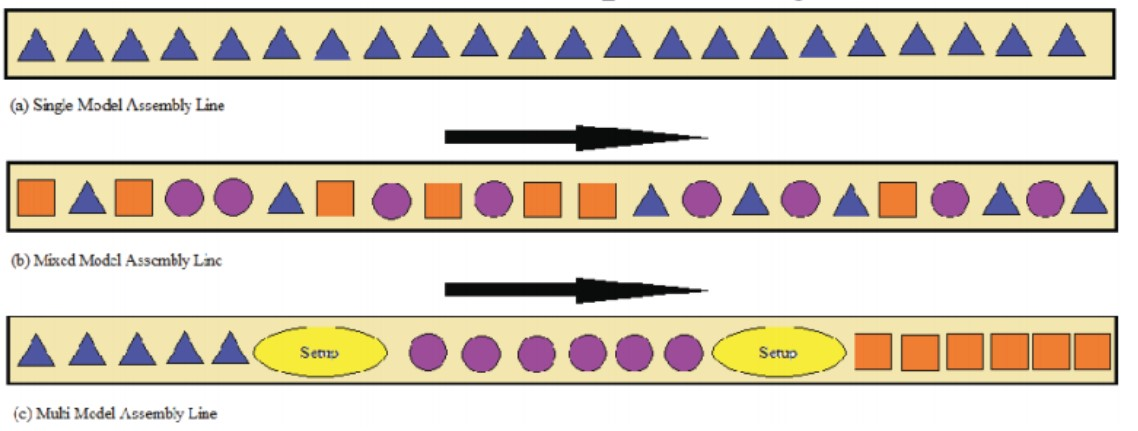
\includegraphics[width=1\linewidth]{fig/Screenshot_2.jpg}}
    \caption{Структура линий из классификации, изображенной на рисунке \ref{ris:image1}}
    \label{ris:shapeOfLines}
\end{figure}

Созданная имитационная модель позволяет игнорировать структурные особенности линии. Основные ограничения, которые невозможно игнорировать включены в технологическую карту. 
\todo[inline, color=red]{Пока непонятно куда девать время предустановки линии в случае MMALBP}

Источник: https://ru.scribd.com/doc/7699063/Introduction-of-Line-Balancing



\section{Обзоры методов решения проблем балансировки линии}

На текущий момент известны множество подходов решения проблемы балансировки линии. Наиболее популярные подходы и методы приведены на рисунке (\ref{ris:Approaches}).

\begin{figure}[H]
    \center{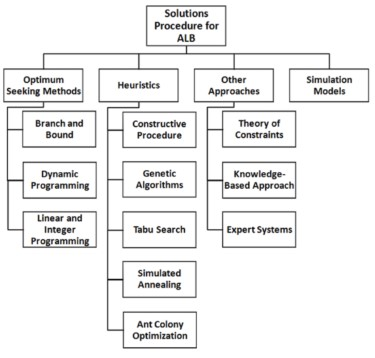
\includegraphics[width=1\linewidth]{fig/Approaches.jpg}}
    \caption{Различные процедуры решения для ALB}
    \label{ris:Approaches}
\end{figure}

Методы оптимального поиска основаны на математических подходах и позволяют найти из множества объектов оптимальный, который соответствует заданным критериям. Одной из основных проблем данного подхода является вычислительная сложность, что в контексте поиска наилучшей конфигурации конвейера, приводит к существенному ограничению использования методов оптимального поиска.

Методы эвристики позволяют избежать проблемы комбинаторной сложности задачи, но при этом результат не всегда будет являться самым оптимальным из возможных. Также эффективность работы алгоритмов эвристики во многом зависят от подхода. На рисунке (\ref{ris:Approaches}) приведены 5 различных эвристических алгоритмов, которые использовались для решения проблемы балансировки линии. Наиболее эффективным из данной группы показал себя генетический алгоритм поиска(ссылка на пруфы). Рассмотрим подробно, как работает генетический алгоритм в контексте балансировки линии.

\subsection{Генетический алгоритм}

Генетические алгоритмы хорошо подходят для решения задач планирования производства, потому что в отличие от эвристических методов генетические алгоритмы работают на совокупности решений, а не на одном решении. В производственном планировании эта совокупность решений состоит из множества ответов, которые могут иметь разные, иногда противоречивые цели. Например, в одном решении оптимизировать производственный процесс, который будет завершен за минимальное время. В другом решении оптимизировать для минимального количества дефектов.

По мере того как увеличиваются количество целей, которые пытаемся достичь, также увеличивается количество ограничений на проблему и аналогичным образом увеличиваем сложность. Генетические алгоритмы идеальны для задач такого типа, когда пространство поиска велико, а количество возможных решений мало.

Чтобы применить генетический алгоритм к задаче планирования, необходимо сначала представить каким образом обозначить геном. Одним из способов представления генома планирования является определение последовательности задач и времени начала этих задач относительно друг друга. Каждое задание и соответствующее время его запуска представляют собой ген.

Определенная последовательность задач и времени начала (гены) представляет один ген в нашей популяции. Чтобы убедиться, что геном является возможным решением, надо чтобы он соответствовал ограничениям приоритета. Далее генерируется начальная популяция, используя случайные времена начала в пределах ограничений предшествования. С помощью генетических алгоритмов берется начальная популяция и скрещивается, комбинируя гены с небольшим количеством случайности (мутации). Потомки этой комбинации выбираются на основе фитнес-функции, которая включает одно или много наших ограничений, таких как минимизация времени и минимизация дефектов. Данный процесс продолжаться либо в течение заранее выделенного времени, либо до тех пор, пока не найдется решение, которое соответствует минимальным критериям. В целом каждое последующее поколение будет иметь более высокую среднюю пригодность, то есть займет меньше времени с более высоким качеством, чем предыдущие поколения. При планировании задач, как и в случае с другими решениями генетического алгоритма, необходимо убедиться, что мы не выбираются недопустимые потомки, такие как отпрыски, которые нарушают наше ограничение приоритета. Также может потребоваться добавить дополнительные значения пригодности, такие как минимизация затрат; однако каждое добавляемое ограничение значительно увеличивает пространство поиска и уменьшает количество подходящих решений.